\section{Tilpasning af træningsniveau}
I tilpasningscontrolleren beregnes den anbefalede træningstid. Dette gøre ud fra kategorisering, den daglige helbredstilstand og en tidligere evaluering, foretaget efter samme træningsform, -type og helbredstilstand.
Beregningen for den anbefalede træning er implementeret ved brug af if/else statement. Et udpluk af denne beregning fremgår af \autoref{fig:anbekode}.  
   
\begin{figure} [H]
\centering
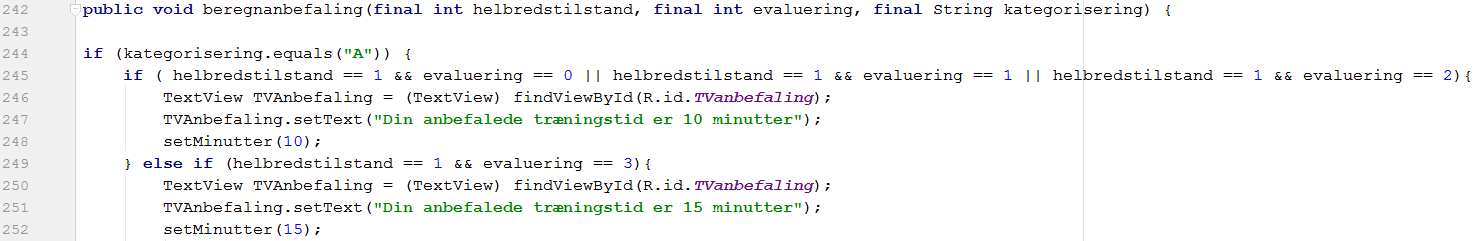
\includegraphics[width=1\textwidth]{figures/imple/anbekode}
\caption{Udpluk af koden for anbefalet træning. If/else loops afgør, hvilket træningsniveau brugeren får anbefalet.}
\label{fig:anbekode}
\end{figure} 

\noindent
Af figuren ses beregningen af den anbefalede træningstid for brugeren med kategorisering \textit{A} og heldbredstilstanden på \textit{2}. Variationen for anbefalingen afhænger af evalueringen og kan i dette eksempel variere mellem \textit{15}, \textit{20} og \textit{25}  minutter. Metodekaldet \textit{setMinutter} referer til, at der sættes en bemærkning idet den anbefaldede træningstid er opnået.

\section{Træning}
Træningscontrolleren har til formål at håndtere GPS og timer under en træning. For at implementere GPS skal app'en have tilladelse til at anvende den mobile enheds lokalisation. Dette er en engangstilladelse, der skal gives første gang brugeren vil foretage en træning. 

Der instansieres en LocationManager og LocationListener. LocationManager tillader app'en at opnå enhedens lokation, hvor LocationListener modtager lokationsopdateringer. Disse opdateringer forekommer, idet enheden ændrer lokation.\cite{} Af koden i \autoref{fig:gpsKode} fremgår det, at systemet indeholder en metode, onLocationChanged, der kaldes, når lokationen ændres. 

\begin{figure} [H]
\centering
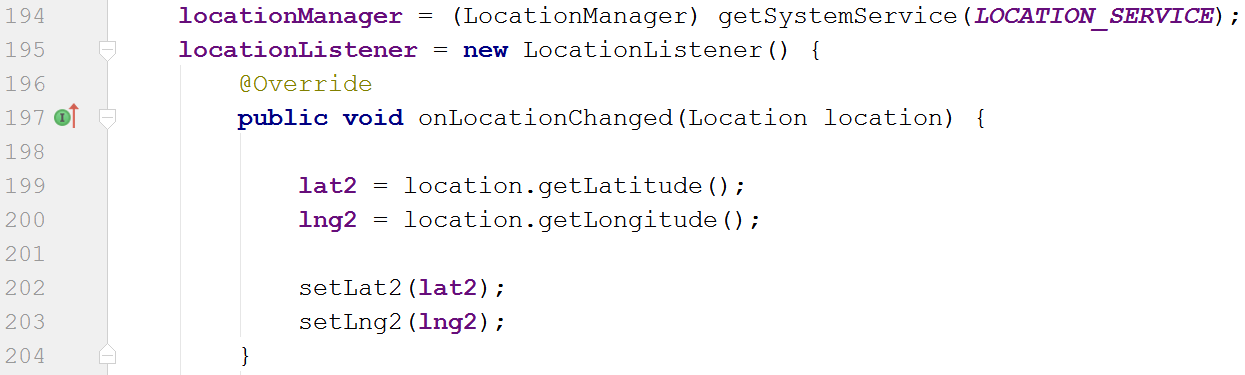
\includegraphics[width=1\textwidth]{figures/imple/gpsKode}
\caption{XXXXXXX.}
\label{fig:gpsKode}
\end{figure} 

Når lokationen ændres, hentes enhedens longitude og latitude, hvortil disse værdier benyttes i set-metoder. 

Der er defineret en metode, der udregner afstanden mellem to lokationer.



https://developer.android.com/reference/android/location/LocationManager.html 

https://developer.android.com/reference/android/location/LocationListener.html

 


GPS:

locationmanager
locationlistener
permission
latitude og longitude
Distance, afstand  + GPS formel
Extended controls


I træningscontrolleren startes en timer. Denne er implementeret ved at instansiere klassen Runnable, hvori en metode, run, defineres. Koden for dette kan ses i \autoref{fig:timerKode}.

\begin{figure} [H]
\centering
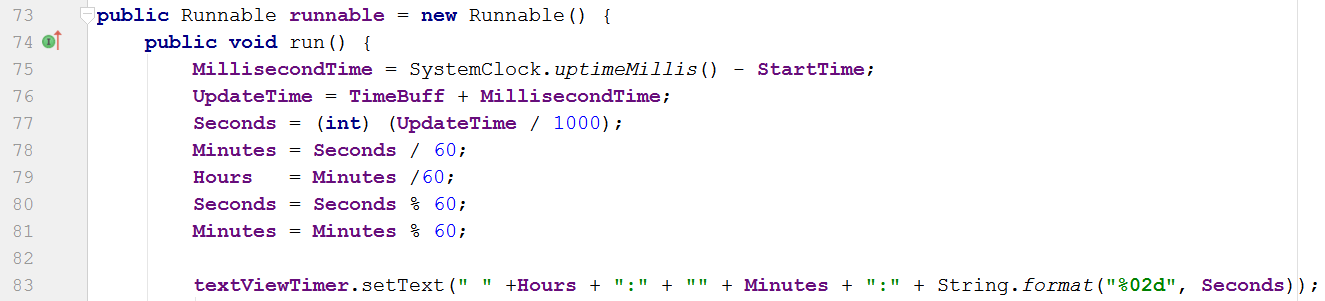
\includegraphics[width=1\textwidth]{figures/imple/timerKode}
\caption{Udklip af kode fra træningscontrolleren. Udklippet viser metoden for timeren.}
\label{fig:timerKode}
\end{figure} 

\noindent
Metoden, run, indeholder variablen MillisecondTime, der tæller tiden, som er gået siden brugeren har trykket start træning. Vælger brugeren at trykke stop træning, stopper MillisecondTime med at tælle op, hvortil denne værdi gemmes i variablen TimeBuff.  Værdien gemmes for at timer vil kunne fortsætte, hvis brugeren fortryder at have stoppet træningen. Seconds defineres ud fra UpdateTime, der måles i millisekunder. Det defineres yderligere, at Seconds kun kan tælle op til 60.

Under tilpasning af træningsniveau er der blevet anbefalet en træningstid. Opnår træningstiden denne værdi under træning, vil app'en gøre brugeren opmærksom på dette ved angivelse af en lyd. Dette er implementeret ved en if-loop, hvori klassen MediaPlayer instansieres, hvis den anbefalede tid opnås. Hertil kaldes en metode, der afspiller en lydfil. 

Ifølge de opstillede kravspecifikationer skal app'en sende en daglig notifikation. Denne er implementeret i træningscontrolleren, hvor notifikationen aktiveres første gang brugeren har evalueret en træning. Hertil er det implementeret, at den daglige notifikation sendes klokken 15. Af \autoref{fig:notifikationKode} fremgår et udklip af koden, som definerer tidspunktet for notifikationen. 

\begin{figure} [H]
\centering
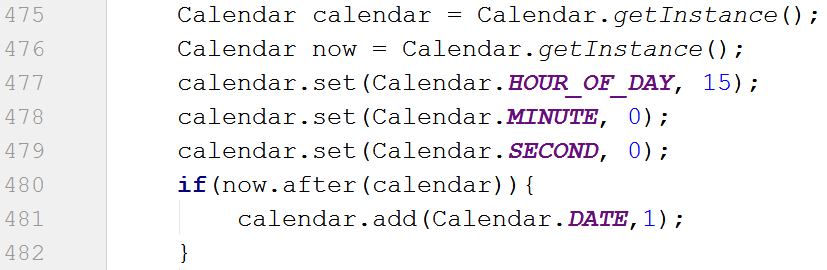
\includegraphics[width=1\textwidth]{figures/imple/notifikationKode}
\caption{Udklip af kode fra træningscontrolleren, som viser notifikationens starttidspunkt.}
\label{fig:notifikationKode}
\end{figure} 







